\chapter{Método PRISMA para revisão bibliográfica}

Este apêndice descreve a metodologia de revisão sistemática utilizada para pesquisar as referências bibliográficas utilizadas neste trabalho. O método utiliza 9 etapas, baseadas no \textit{framework} PRISMA \cite{Moher2010}. Estas etapas são: 1) definição do tópico de pesquisa, 2) definição dos conceitos envolvidos, 3) seleção das fontes bibliográficas, 4) definição dos termos de busca, 5) definição da estratégia de pesquisa, 6) critérios de seleção e 7) construção do diagrama de fluxos. Cada um dos passos citados será mostrado como se segue:

\section{Definição do tópico de pesquisa}\label{sec:prisma_topico} 

Esta etapa especificou o tópico que orientou a definição dos conceitos envolvidos nesta pesquisa. O tópico de pesquisa escolhido foi: ``Redução de dados em fluxos de dados com mudança de conceito''.

\section{Definição dos conceitos envolvidos }\label{sec:prisma_conceitos} 

Com base na pesquisa de definição de tópicos, foram identificados três conceitos envolvidos: 1) \textit{Data Streams}; 2) \textit{Concept Drift}; 3) \textit{Data Reduction}. Esses conceitos serão descritos a seguir:

\begin{itemize}
\item \textit{Data Streams}: é uma sequência ordenada e potencialmente infinita de instâncias, transmitidas em alto volume e alta velocidade, o que impede seu completo armazenamento em memória. Diante desses fatores, tais instâncias precisam ser analisadas em tempo real.
\item \textit{Concept Drift}: É uma mudança inesperada na relação de um conjunto de variáveis $X$ a uma saída $y$ durante um intervalo de tempo. A definição formal é dada por: $ \exists X : p_t0 (X,y) \neq p_t1 (X,y) $ e.g. dados de sensores usados para captação de abalos sísmicos podem variar inesperadamente em caso de um princípio de terremoto.
\item \textit{Data Reduction}: técnicas de pré-processamento que visam reduzir um determinado conjunto de dados à uma representação menor em volume, porém mantendo a qualidade estatística das informações. Essas técnicas podem ser usadas tanto para reduzir as instâncias quanto os atributos do conjunto de dados.
\end{itemize}

\section{Seleção das fontes bibliográficas }\label{sec:prisma_fontes} 

As pesquisas foram realizadas nas bases IEEE Xplore, Science Direct, ACM Digital Library e Web of Science. Pesquisas manuais em bibliotecas, bem como artigos indicados pelo orientador ou outros especialistas foram realizadas em paralelo. Os artigos, livros ou dissertações/teses obtidas por esses meios não serão descritos neste apêndice.

\section{Definição dos termos de busca}\label{sec:prisma_termos} 

Os termos de pesquisa foram especificados pela observação das palavras-chave pertinentes à este trabalho e por indicações do orientador. Assim, os termos de pesquisa utilizados foram:  1) \textit{Data Streams}; 2) \textit{Concept Drift} e 3) \textit{Data Reduction}. No IEEE Xplore, a pesquisa foi realizada com base no campo ``Full Text and Metadata''. No ScienceDirect, não foi especificado nenhum campo, para que a pesquisa abrangesse todos os textos na íntegra. Na ACM Digital Library, também não foi selecionado nenhum campo específico. Na base Web of Science, foi selecionada a aba ``Advanced Search'', utilizando a busca por tópico (\textit{topic search} -- TS). 

\section{Definição da estratégia de pesquisa}\label{sec:prisma_estrategia} 

Um exemplo de estratégia de pesquisa no ScienceDirect pode ser vista na Tabela~\ref{tab_estr_pesquisa} a seguir.

\begin{table}[!htp]
\centering
\caption{Exemplo de estratégia de pesquisa para ScienceDirect e número de \textit{hits} retornados}

\label{tab_estr_pesquisa}
\begin{tabular}{|l|}
\hline
\begin{tabular}[c]{@{}l@{}}\textbf{1. Data Streams (18,882)}\\ (``Data Streams'')\end{tabular}                                                                   \\ \hline
\begin{tabular}[c]{@{}l@{}}\textbf{2. Concept Drift (548)}\\ (``Concept Drift'')\end{tabular}                                                                    \\ \hline
\begin{tabular}[c]{@{}l@{}}\textbf{3. Data Reduction (60,451)}\\ (``Data Reduction'')\end{tabular}                                                                    \\ \hline
\begin{tabular}[c]{@{}l@{}}\textbf{4. Pesquisa Final (889)}\\ \textbf{( 1  AND 2 ) OR (1 AND 3 )}\\ (``Data Streams'' AND ``Concept Drift'') OR (``Data Streams'' AND ``Data Reduction'')\end{tabular} \\ \hline
\end{tabular}
\end{table}

Após a realização da pesquisa, um gráfico com a quantidade de publicações por ano foi gerado, como pode ser visto na Figura~\ref{fig:referencias}.

\begin{figure}[!htb]
\centering
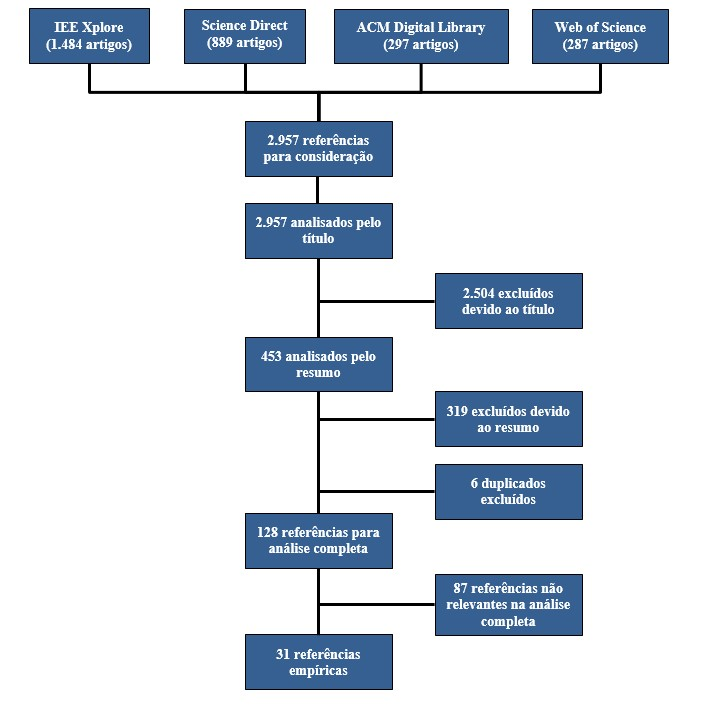
\includegraphics[scale=0.8]{referencias.jpg}
\caption{Revisão Sistemática}
\label{fig:referencias}
\end{figure}

\section{Critérios de Seleção}\label{sec:prisma_criterios} 

Após a execução da pesquisa, cada artigo foi submetido a um conjunto de critérios de elegibilidade, visando a obtenção dos artigos que fossem pertinentes a este trabalho. Todos aqueles que não se enquadraram nos critérios estabelecidos foram excluídos. Os critérios utilizados para avaliação dos artigos nas etapas de título inicial e resumo foram: o assunto é lidar com \textit{Concept Drift} e/ou \textit{Data Reduction} em \textit{Data Streams}. Sendo assim, foram definidos os seguintes critérios:
\begin{itemize}
\item É uma proposta ou implementação de algoritmo de redução de dados em\textit{Data Streams};
\item É uma proposta ou implementação para lidar com o fenômeno de \textit{Concept Drift} em \textit{Data Streams};
\item É uma pesquisa recente ou referência teórica.
\end{itemize}

Quanto a etapa de leitura completa do texto, os critérios utilizados foram:

\begin{itemize}
\item análise do método utilizado;
\item análise dos resultados;
\item análise de contribuição relevante.
\end{itemize}

Ao final, uma análise completa e detalhada de cada um dos artigos selecionados a partir dos critérios acima especificados foi realizada. Os resultados obtidos durante essa análise foram utilizados para compor a Tabela~\ref{tab_pontos-chave_artigos}, que apresenta os principais pontos de cada artigo selecionado. Os detalhes são apresentados a seguir.

\section{Diagrama de Fluxo}\label{sec:prisma_diagrama} 

As primeiras pesquisas resultaram em 2.957 referências, 31 das quais foram selecionadas por cumprirem os critérios de elegibilidade, de acordo com a Figura~\ref{fig:referencias}. As características dessas 31 referências e seus pontos chave são apresentados na Tabela~\ref{tab_pontos-chave_artigos}. 



\begin{longtable}[c]{|p{2.7cm}|p{5cm}|p{7cm}|}
\caption{Referências levantadas e seus pontos-chave}
\label{tab_pontos-chave_artigos}
\\ \hline
\textbf{Autor (ano)}            & \textbf{Título da referência}                                                                                                   & \textbf{Pontos Chave}                                                                                                                                                     
\\
\endfirsthead  

\multicolumn{3}{c}%
{{\tablename\ \thetable{} -- continuação da página anterior}} \\
\hline
\textbf{Autor (ano)}            & \textbf{Título da referência}                                                                                                   & \textbf{Pontos Chave}                                                                                                                                                     
\\
\endhead

\hline \multicolumn{3}{|r|}{{Continua na próxima página...}} \\ \hline
\endfoot

\endlastfoot

\hline
\cite{Goncalves2014}  & A comparative study on concept drift detectors & Artigo com um estudo comparativo entre detectores de concept drift, que apresenta vários tipos existentes e seus desempenhos diante de alguns critérios. Apresenta datasets importantes e previamente utilizados na área de concept drift.         
\\ \hline
\cite{Carmona-Cejudo2013} & A comparative study on feature selection and adaptive strategies for email foldering using the ABC-DynF framework & Artigo que apresenta um estudo de caso ao aplicar técnicas de seleção de atributos como etapa de pré-processamento para otimização do processo de classificação no armazenamento automático de e-mails (email foldering).
\\ \hline
\cite{Wankhade2013} & A new feature selection algorithm for stream Data Classification & Artigo que apresenta um algoritmo de seleção de atributos híbrido, baseado em Informação Mutúa e Algoritmos Genéticos, para otimização do processo de classificação de data streams.
\\ \hline
\cite{Siddiqa2016} & A survey of big data management: Taxonomy and state-of-the-art & Artigo que apresenta o estado da arte e a taxonomia dos principais conceitos que envolvem Big Data.
\\ \hline
\cite{Gama2014} & A survey on concept drift adaptation & Artigo escohido por ser uma das referências mais utilizadas quanto à conceituação do que é concept drift, quais tipos existem e como detectá-los. Têm como autor principal um dos pesquisadores mais conceituados da área, João Gama.
\\ \hline
\cite{Ramirez-Gallego2017} & A survey on data preprocessing for data stream mining: Current status and future directions & Artigo escolhido por trazer o estado da arte das técnicas de pré-processamento em data streams.
\\ \hline
\cite{Barddal2017} & A survey on feature drift adaptation: Definition, benchmark, challenges and future directions & Artigo selecionado por descrever definições e trazer o estado da arte dos algoritmos e técnicas de adaptações às mudanças nos atributos em data streams.
\\ \hline
\cite{Bolon-Canedo2016} & A unified pipeline for online feature selection and classification & Artigo selecionado por trazer um algoritmo de seleção de atributos que atua juntamente com um classificador de data streams.
\\ \hline
\cite{Singh2015} & An intrusion detection system using network traffic profiling and online sequential extreme learning machine & Artigo que apresenta uma técnica de detecção de intrusos em uma rede online à partir de diversos métodos, incluindo a utilização de seleção de atributos nos dados recebidos. Os autores utilizam um dataset que pode ser utilizado no trabalho.
\\ \hline
\cite{Barddal2015} & Analyzing the Impact of Feature Drifts in Streaming Learning & Artigo que apresenta o impacto das mudanças de atributos em data streams no processo de aprendizado online. Os autores apresentam um gerador de fluxos para simulação deste tipo de occorrência.
\\ \hline
\cite{Cassidy2014} & Calculating feature importance in data streams with concept drift using Online Random Forest & Artigo que apresenta um método ( Online Random Forest) para calcular a importância de atributos em data streams, inclusive aqueles que contém concept drift. Também apresenta um dataset importante na área de concept drift, o Hyperplane Dataset.
\\ \hline
\cite{Garcia-Osorio2010} & Democratic instance selection: A linear complexity instance selection algorithm based on classifier ensemble concepts & Artigo que apresenta uma outra técnica de redução de dados, Instance Selection, utilizada para reduzir instâncias ao invés de atributos. Apresenta diversos datasets interessantes que podem ser utilizados no trabalho.
\\ \hline
\cite{Turkov2016} & Feature Selection for Handling Concept Drift in the Data Stream Classification & Artigo que apresenta uma proposta em utilizar seleção de atributos para lidar com concept drift em data streams. No estudo experimental, apresenta a técnica utilizada para gerar datasets artificiais com concept drift e alta dimensionalidade, incluindo atributos irrelevantes.
\\ \hline
\cite{Yue2008} & Immune-inspired incremental feature selection technology to data streams & Artigo que apresenta um algoritmo imuno-inspirado para seleção de atributos em data streams.
\\ \hline
\cite{Wang2016} & Improved Data Streams Classification with Fast Unsupervised Feature Selection & Esse artigo apresenta um estudo de como a seleção de atributos otimiza o processo de de classificação em data streams.
\\ \hline
\cite{Stiglic2011} & Interpretability of Sudden Concept Drift in Medical Informatics Domain & Artigo selecionado por apresentar um dataset com concept drift e um método de visualização para comprovar a existência de concept drift que pode ser útil neste trabalho.
\\ \hline
\cite{Li2015} & Learning concept-drifting data streams with random ensemble decision trees & Artigo que apresenta a aplicação de um ensemble de árvores de decisão em data streams com concept drift. Apresenta datasets que podem ser utilizados neste trabalho.
\\ \hline
\cite{Jankowski2016} & Learning Decision Trees from Data Streams with Concept Drift & Artigo que apresenta a aplicação de um árvore de decisão em data streams com concept drift. Apresenta datasets que podem ser utilizados neste trabalho.
\\ \hline
\cite{Gomes2014} & Mining Recurring Concepts in a Dynamic Feature Space & Artigo que apresenta um método para lidar com concept drifts recorrentes em um ambiente em que os atributos mudam com o tempo.
\\ \hline
\cite{Bifet2009} & New ensemble methods for evolving data streams & Artigo que apresenta geradores e simuladores de data streams com concept drift e algumas informações pertinentes sobre esse fenômeno.
\\ \hline
\cite{Razmjoo2017} & Online feature importance ranking based on sensitivity analysis & Artigo que apresenta um método de seleção de atributos em data streams.
\\ \hline
\cite{Chen2011} & Online fractal dimensionality reduction in time decaying stream environment & Artigo que apresenta uma técnica de redução de dados conhecida como Online Fractal Dimensionality Reduction aplicada à streams. Contém datasets interessantes e que podem ser utilizados.
\\ \hline
\cite{Rajput2014} & Optimize Intrusion Prevention and Minimization of Threats for Stream Data Classification & Artigo que apresenta a implementação de um sistema de detecção de intrusos com aplicação de técnica de seleção de atributos baseado em algoritmo genético.
\\ \hline
\cite{Hosseini2011} & Pool and Accuracy Based Stream Classification: A New Ensemble Algorithm on Data Stream Classification Using Recurring Concepts Detection & Artigo que apresenta datasets importantes com concept drift, incluindo recorrentes, graduais e repentinos.
\\ \hline
\cite{MiguelAngel2016} & Predicting recurring concepts on data-streams by means of a meta-model and a fuzzy similarity function & Artigo que discorre sobre o concept drift recorrente e os meios possíveis de se prever a ocorrência dos mesmos. Útil para referências sobre esse tipo de concept drift.
\\ \hline
\cite{GoncalvesJr2013} & RCD: A recurring concept drift framework & Artigo que apresenta um framework para lidar com concept drifts recorrentes. O mesmo foi testado em datasets reais e artificiais que podem ser utilizados neste trabalho.
\\ \hline
\cite{Barros2017} & RDDM: Reactive Drift Detection Method & Artigo que apresenta um detector de drift testado em diferentes datasets reais e artificiais com diferentes tipos de concept drift que podem ser utilizados neste trabalho.
\\ \hline
\cite{Bolon-Canedo2015} & Recent advances and emerging challenges of feature selection in the context of big data & Artigo que apresenta os avanços e os desafios da área de seleção de atributos no contexto de Big Data, incluindo estudos e algoritmos existentes em data streams.
\\ \hline
\cite{Zhou2005} & Streaming feature selection using alpha-investing & Artigo que apresenta um aprimoramento do algoritmo Streaming Feature Selection (SFS) e pode trazer novas ideias para o trabalho.
\\ \hline
\cite{Zhang2017} & Three-layer concept drifting detection in text data streams & Estudo que apresenta, dentre outros aspectos, os tipos de concept drift que podem acontecer no campo de mineração de texto em data streams.
\\ \hline
\cite{Huang2015} & Unsupervised Feature Selection on Data Streams & Artigo que apresenta um algoritmo de seleção de atributos não supervisionado em data streams, que funciona inclusive na presença de concept drifts.
\\ \hline
\end{longtable}

\chapter{Configurações de projeto e instruções de uso} \label{chp:ApendiceB}

Até a 
elaboração deste texto
, dois dos seis algoritmos propostos para a avaliação foram implementados. Esses algoritmos foram construídos em um projeto de aplicação Java, utilizando a IDE Eclipse, e compactados em um arquivo ``.jar'' para serem utilizados como uma extensão da ferramenta MOA. O projeto pode ser visualizado no repositório Github construído para este trabalho \cite{githubMbdemoraes}.

Para execução do projeto como uma extensão do MOA, o arquivo ``.jar'' dever ser adicionado dentro da pasta ``lib'', localizado no diretório onde o MOA está instalado. A partir disso, o usuário deve acessar o \textit{prompt} ou terminal de comando de seu sistema operacional, navegar até o diretório raiz do \textit{framework} MOA e executar o seguinte comando (onde nome\_do\_arquivo representa o nome gerado após a exportação do projeto Java no formato .jar):


\begin{itemize}
\item \textbf{Windows}: \texttt{java -cp .;lib/nome\_do\_arquivo.jar;moa.jar;lib/weka.jar}\smallbreak \texttt{-javaagent:sizeofag-1.0.0.jar moa.gui.GUI}
\item \textbf{Linux}: \texttt{java -cp lib/nome\_do\_arquivo.jar:moa.jar:lib/weka.jar} \smallbreak \texttt{-javaagent:sizeofag-1.0.0.jar moa.gui.GUI}
\end{itemize}

Antes da realização dos experimentos, o MOA deve ser configurado com os parâmetros específicos. A Figura~\ref{fig:configuracao_moa} mostra a tela de configuração construída para este projeto. Para acessá-la, o usuário deve selecionar a aba Classification -> botão Configure -> na tela seguinte, no campo Learner, clicar no botão Edit -> na lista de opções apresentadas, selecionar: class moa.featureselection.classifiers.NaiveBayes.

\begin{figure}[!htb]
  \centering
    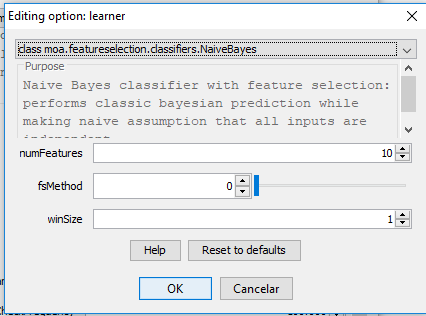
\includegraphics[width=.8\textwidth]{configuration_moa.png}
    \caption{Tela de configurações do MOA para execução dos experimentos.}
    \label{fig:configuracao_moa}
\end{figure}

Neste tela, o usuário possui três opções de configuração, descritas a seguir:

\begin{itemize}
\item \textit{numFeatures}: quantidade de atributos que o algoritmo de seleção de atributos deve selecionar ao fina de sua execução.
\item \textit{fsMethod}: algoritmo de seleção de atributos à ser avaliado. A opção 0, padrão, indica que nenhuma seleção de atributos será aplicada. Desse modo, o classificador utilizará todos os atributos contidos nos fluxos. A opção 1 é para utilização do Método de Katakis com Ganho de Informação. Opção 2 para utilização do FCBF e, por fim a opção 3 para utilização do algoritmo OFS.
\item \textit{winSize}: janela de processamento. Define quantos fluxos serão processados por vez. O padrão é 1.
\end{itemize}